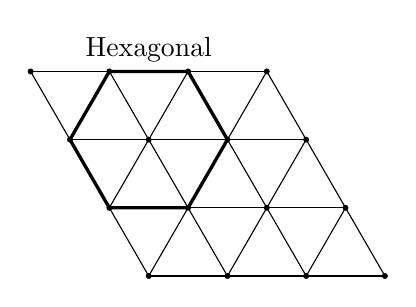
\begin{tikzpicture}[scale=1]

%draw the hexagonal lattice
\coordinate (hexagonal) at (2,2.6);
\node [above] at (hexagonal) {Hexagonal}; %Couldn't figure out an elegant way to do the hexagonal lattice - TWJ 6/14/2010

\draw (2,0) -- (5,0);
\draw (1.5,0.866) -- (4.5,0.866);
\draw (1,1.732) -- (4,1.732);
\draw (0.5,2.598) -- (3.5,2.598);
\draw (2,0) -- (0.5,2.598);
\draw (3,0) -- (1.5,2.598);
\draw (4,0) -- (2.5,2.598);
\draw (5,0) -- (3.5,2.598);
\draw (2,0) -- (3.5,2.598);
\draw (3,0) -- (4,1.732);
\draw (4,0) -- (4.5,0.866);
\draw (1.5,0.866) -- (2.5,2.598);
\draw (1,1.732) -- (1.5,2.598);
\draw [very thick] (1.5,0.866) -- (1,1.732) -- (1.5,2.598) -- (2.5,2.598) -- (3,1.732) --  (2.5,0.866) -- cycle;
\foreach \x in {2,3,4,5} \filldraw[fill=black, draw=black] (\x,0) circle (0.03);
\foreach \x in {1.5,2.5,3.5,4.5} \filldraw[fill=black, draw=black] (\x,0.866) circle (0.03);
\foreach \x in {1,2,3,4} \filldraw[fill=black, draw=black] (\x,1.732) circle (0.03);
\foreach \x in {0.5, 1.5,2.5,3.5} \filldraw[fill=black, draw=black] (\x,2.598) circle (0.03);

\end{tikzpicture}

